\section{COFF}

\begin{frame}[t]{COFF}{Common Object File Format}
    \begin{columns}
    \column{.5\textwidth}
    \begin{itemize}
        \item ELF
        \item PE(Protable Executable)
        \begin{itemize}
            \item x86: Support NT, 95, XP, Vista, CE
            \item 64bit: PE32+
            \item custom sections
        \end{itemize}
        \item Default object file format of Visual C++: COFF
    \end{itemize}
    \column{.5\textwidth}
        \begin{figure}
            \begin{center}
                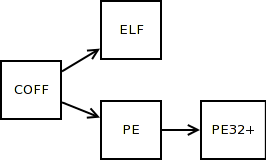
\includegraphics[width=\textwidth]{./image/COFF.png}
                \caption{COFF, ELF, PE and PE32+}
            \end{center}
        \end{figure}
    \end{columns}
\end{frame}


\begin{frame}[fragile]{Custom Section}
    \begin{lstlisting}
#pragma data_seg("FOO")
int global = 1;
#pragma data_seg(".data")
    \end{lstlisting}
    \begin{block}{\#pragma}
        \begin{itemize}
            \item line1 \#pragma之後的全域變數放進"FOO" section
            \item line3 \#再切換回來放進去預設的".data" section
        \end{itemize}
    \end{block}
\end{frame}


\begin{frame}[t]{Visual C++}
    \begin{columns}
    \column{.5\textwidth}
    \begin{itemize}
        \item Compiler: \emph{cl}
        \item Linker: \emph{link}
        \item COFF Binary Dump tool: \emph{dumpbin}
        \item Visual C++ Express 2010(Free)\\
            \href{http://www.microsoft.com/visualstudio/cht/downloads\#d-2010-express}{\color{blue}{\emph{download link}}}
    \end{itemize}
    \column{.5\textwidth}
    \begin{figure}
        \begin{center}
            
\includegraphics[width=.7\textwidth]{./image/Visual-C++-2010-Express.jpg}
        \end{center}
    \end{figure}
\end{columns}
\end{frame}

\begin{frame}[fragile]{Complie with VC++}
        \begin{lstlisting}
cl /c /Za SimpleSection.c

dumpbin /ALL SimpleSection.obj > SimpleSection.txt
dumpbin /SUMMARY SimpleSection.obj
        \end{lstlisting}
        \begin{block}{\emph{cl}}
        \begin{itemize}
            \item /c: compile only
            \item /Za:  停用擴充功能
        \end{itemize}
        \end{block}
        \begin{block}{\emph{dumpbin}}
        \begin{itemize}
            \item /ALL: 輸出obj 所有相關資訊
            \item /SUMMARY: 輸出obj 基本資訊
        \end{itemize}
        \end{block}
\end{frame}


\begin{frame}[t]{COFF Object File Format}
    \begin{columns}[t]
        \column{.4\textwidth}
        \begin{itemize}
            \item Image File Header
            \item Image Section Header
            \item Sections
            \begin{itemize}
                \item \emph{.text}
                \item \emph{.data}
                \item \emph{.debug\$S}
            \end{itemize}
            \item Symbol Table
            \item "VC\textbackslash PlatformSDK \textbackslash include \textbackslash \textbf{WinNT.h}"
        \end{itemize}
        \column{.4\textwidth}
        \begin{figure}
            \begin{center}
                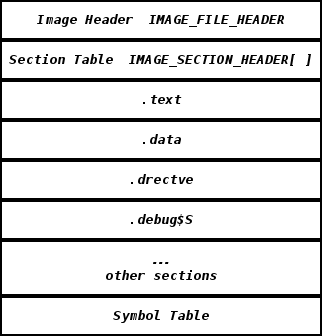
\includegraphics[width=\textwidth]{./image/COFFObjFormat.png}
                \caption{COFF File Format}
            \end{center}
        \end{figure}
    \end{columns}
\end{frame}

\begin{frame}{Image File Header}
    \begin{columns}[t]
        \column{.4\textwidth}
        \begin{figure}
            \begin{center}
                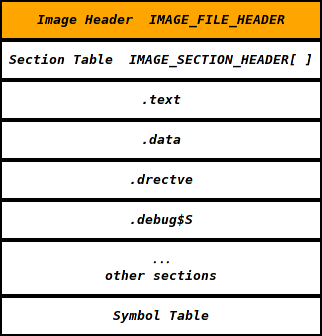
\includegraphics[width=.5\textwidth]{./image/imagefileheader.png}
            \end{center}
        \end{figure}
        \column{.6\textwidth}
        \begin{figure}
            \begin{center}
                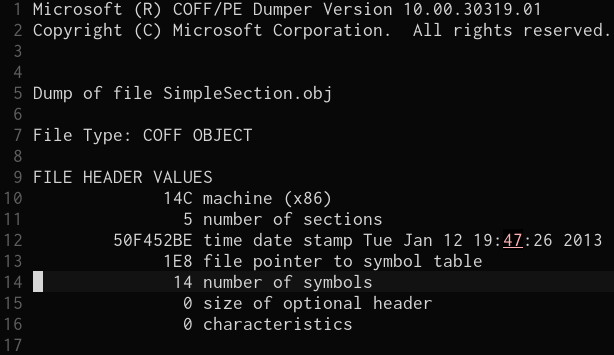
\includegraphics[width=\textwidth]{./image/objimghdr.png}
                \caption{image file header information}
            \end{center}
        \end{figure}
    \end{columns}
\end{frame}

\begin{frame}{Image Section Header}
    \begin{columns}[t]
        \column{.4\textwidth}
        \begin{figure}
            \begin{center}
                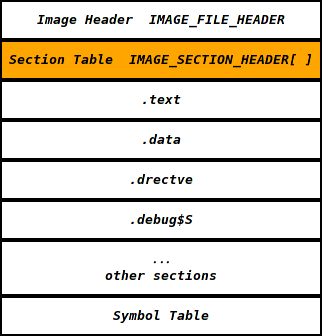
\includegraphics[width=.5\textwidth]{./image/imagesectionheader.png}
            \end{center}
        \end{figure}
        \column{.6\textwidth}
        \begin{figure}
            \begin{center}
                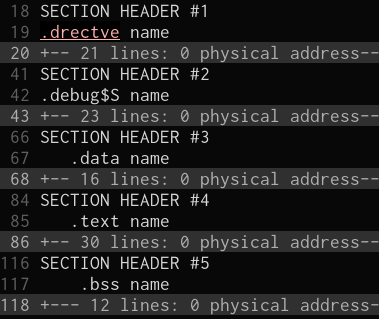
\includegraphics[width=.75\textwidth]{./image/imgsechdr.png}
                \caption{image section header information}
            \end{center}
        \end{figure}
    \end{columns}
\end{frame}

\begin{frame}[t]{Section Attributes}
    \begin{itemize}
        \item name
        \item virtual size/addr
        \item size of raw data
        \item characteristics
    \end{itemize}
\end{frame}


\begin{frame}{.drectve section}{連結指示資訊}
    \begin{columns}[t]
        \column{.5\textwidth}
        \begin{figure}
            \begin{center}
                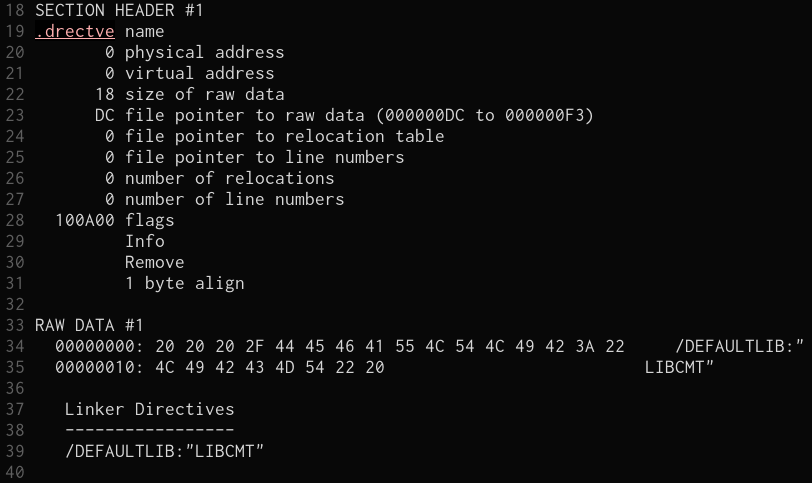
\includegraphics[width=\textwidth]{./image/directivesec.png}
            \end{center}
        \end{figure}
        \column{.5\textwidth}
        \begin{itemize}
            \item name: Directive 的縮寫
            \item Characteristics: 0x100A00
            \item 0x100A00 = 0x100000 + 0x800 + 0x200 \\
                  p.140 表5-2
            \item LIBCMT: Library C Multithreaded, 表示\\\textbf{靜態連結的多緒程C函式庫}
        \end{itemize}
    \end{columns}
\end{frame}

\begin{frame}{.debug section}{除錯資訊}
    \begin{columns}[t]
        \column{.5\textwidth}
        \begin{figure}
            \begin{center}
                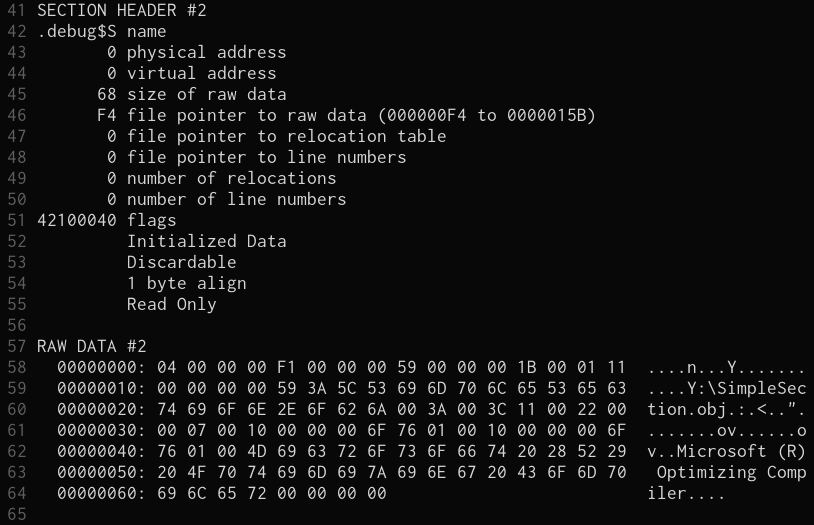
\includegraphics[width=\textwidth]{./image/debugsec.png}
            \end{center}
        \end{figure}
        \column{.5\textwidth}
        \begin{itemize}
            \item name:
            \begin{itemize}
            \item .debug\$S(symbol contained)
            \item .debug\$P(precompiled header files contained) 
            \item .debug\$T(type contained)
            \end{itemize}
        \end{itemize}
    \end{columns}
\end{frame}


\begin{frame}{Symble Table}
    \begin{columns}[t]
        \column{.5\textwidth}
        \begin{figure}
            \begin{center}
                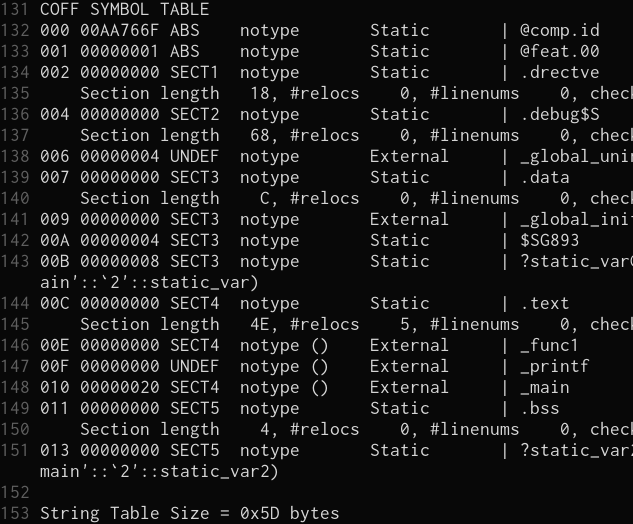
\includegraphics[width=\textwidth]{./image/symboltablesec.png}
                \caption{COFF symbol table}
            \end{center}
        \end{figure}
        \column{.5\textwidth}
        \begin{itemize}
            \item column1: index
            \item column2: size
            \item column3: position
            \begin{itemize}
                \item section number: SECT1, SECT2 ...
                \item global: ABS
            \end{itemize}
            \item column4: type(notype/notype ()), 可供強弱符號運用
            \item column5: scope
            \begin{itemize}
                \item External: 全域
                \item Static: 區域
            \end{itemize}
            \item column6: symbol name
            \item String Table Size
        \end{itemize}
    \end{columns}
\end{frame}

%-------

\section{PE}
\begin{frame}
    \begin{columns}[t]
        \column{.5\textwidth}
        \begin{itemize}
            \item COFF extension
            \item 2 major differeces
            \begin{enumerate}
                \item Started by \textbf{DOS MZ File Header and Stub}
                    compitible with MZ(old DOS .exe file format)
                \item \textbf{IMAGE\_NT\_HEADERS}
            \end{enumerate}
            \item IMAGE\_DOS\_HEADER:
            \begin{itemize}
                \item "e\_cs, e\_ip", point to "DOS Stub"
                \item "This program cannot be run in DOS"
                \item \textbf{"e\_lfanew"}
                \begin{itemize}
                    \item MZ: 0
                    \item PE: offset to \textbf{IMAGE\_NT\_HEADERS}
                \end{itemize}
            \end{itemize}
        \end{itemize}
        \column{.4\textwidth}
        \begin{figure}
            \begin{center}
                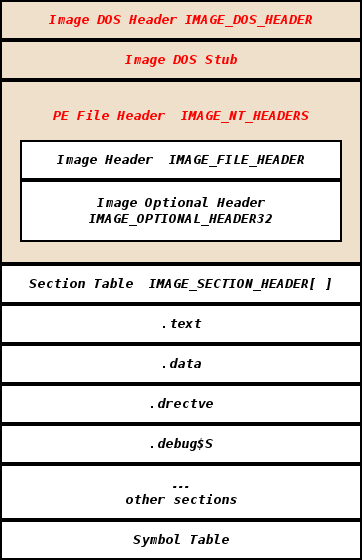
\includegraphics[height=.8\textheight]{./image/PEObjFormat.png}
                \caption{PE File Format}
            \end{center}
        \end{figure}
    \end{columns}
\end{frame}

\begin{frame}[t]{PE File Header}{IMAGE\_NT\_HEADERS}
    \begin{itemize}
        \item PE 真正的HEADER, Optional for COFF, but required for PE-executable file, include DLL files
        \item Signiture: PE\textbackslash 0\textbackslash 0
        \item PE data directory: defined in IMAGE\_OPTIONAL\_HEADER
        \begin{itemize}
            \item 匯入表
            \item 重定表
            \item 資源表
            \item 異常表
            \item 重定表
            \item 除錯資訊表
            \item 緒程私有儲存表(TLS)... 等的位置與長度
        \end{itemize}
        \item WinNT.h
    \end{itemize}
\end{frame}
